\documentclass[a4paper,11pt]{article}

\usepackage[margin=2.5cm]{geometry}
\usepackage{amsmath}
\usepackage[hidelinks]{hyperref}
\usepackage{graphicx}
\usepackage{subcaption}
\usepackage{tabularx}

\title{Mathematical Modelling and Dynamic Response Analysis of a Simplified Vehicle Suspension}
\author{}
\date{}

\begin{document}

\maketitle

\section{Background}

A vehicle suspension connects the vehicle body to the road through elastic and
dissipative elements. Its purpose is to limit the transmission of road-induced
vibration while maintaining acceptable suspension motion. A real suspension
contains tyres, linkages and several distributed masses, but a simpler model is
more suitable for deriving the main dynamic relationships analytically. This
report therefore considers the vertical motion associated with one wheel and
represents the supported part of the vehicle body by a single equivalent mass.
The investigation first derives the governing ordinary differential equation
and its transfer function using Newton's second law and the Laplace transform.
The free response is then used to show how the system poles and damping determine
whether the motion decays with or without oscillation. The same model will later
be used to investigate how a prescribed road displacement is transmitted to the
vehicle body.

% TODO: Add academic sources on suspension modelling and parameter selection.

\section{Description of the Model}

The suspension is represented by a single-degree-of-freedom base-excitation
model. The equivalent sprung mass is connected to a moving lower support by a
linear spring and a viscous damper in parallel, as shown in
Figure~\ref{fig:vehicle}. In this approximation, the lower support follows the
road profile directly.

\begin{figure}[htbp]
    \centering
    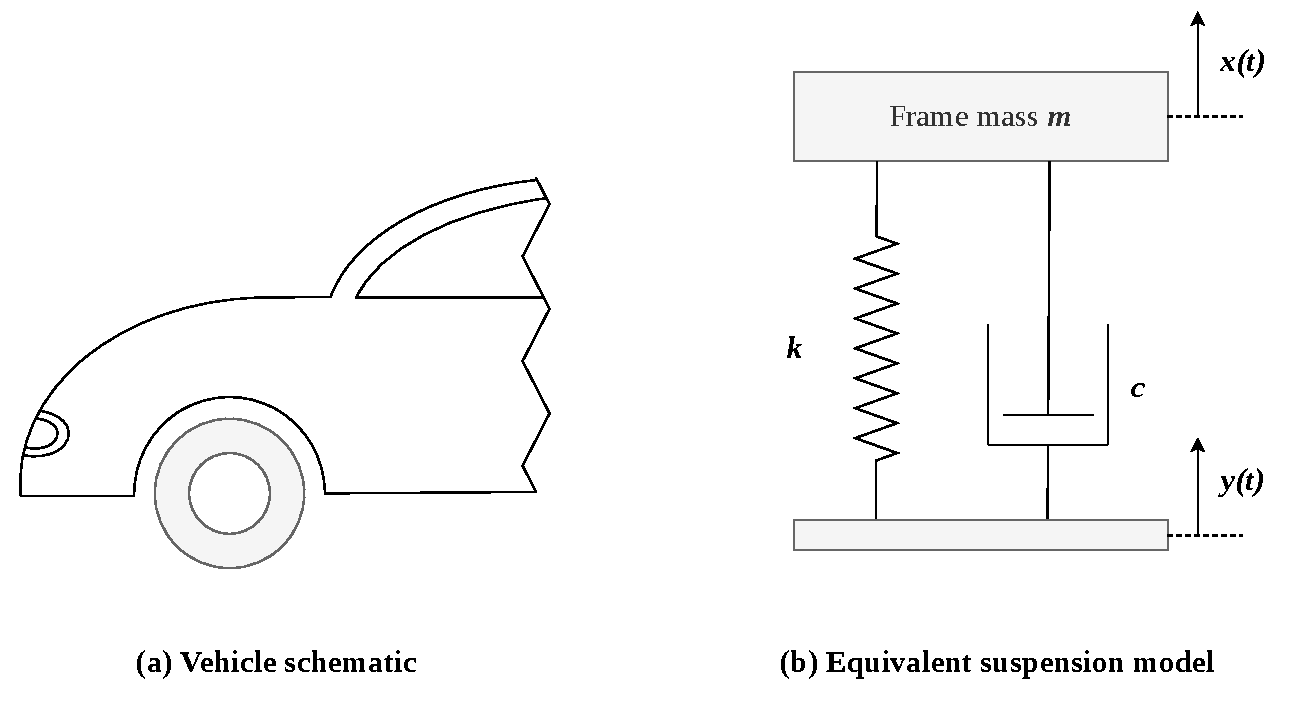
\includegraphics[width=0.68\textwidth]{figures/vehical.pdf}
    \caption{Vehicle schematic and equivalent single-degree-of-freedom suspension model.}
    \label{fig:vehicle}
\end{figure}

\begin{samepage}
The model is based on the following assumptions:
\begin{itemize}
    \item only vertical motion is considered;
    \item the spring and damper are linear;
    \item the wheel mass and tyre deformation are neglected;
    \item the lower support follows the road displacement; and
    \item displacement is measured from static equilibrium, so gravity is
          balanced by the spring preload.
\end{itemize}
\end{samepage}

Both displacements are positive upwards. The variables and parameters are
defined below.

\begingroup
\renewcommand{\arraystretch}{1.2}
\noindent
\begin{tabularx}{\linewidth}{@{}l X l@{}}
    \textbf{Symbol} & \textbf{Meaning} & \textbf{Unit} \\
    \(m\) & Equivalent sprung mass supported by one suspension & \(\mathrm{kg}\) \\
    \(k\) & Spring stiffness & \(\mathrm{N/m}\) \\
    \(c\) & Viscous damping coefficient & \(\mathrm{N\,s/m}\) \\
    \(x(t)\) & Vehicle-body displacement from static equilibrium & \(\mathrm{m}\) \\
    \(y(t)\) & Road or lower-support displacement & \(\mathrm{m}\) \\
    \(F_k\) & Incremental spring force on the mass & \(\mathrm{N}\) \\
    \(F_c\) & Incremental damping force on the mass & \(\mathrm{N}\) \\
\end{tabularx}
\endgroup

The spring force depends on relative displacement, whereas the damping force
depends on relative velocity:
\[
    F_k=-k(x-y),
    \qquad
    F_c=-c(\dot{x}-\dot{y}).
\]
Newton's second law therefore gives
\[
    m\ddot{x}=F_k+F_c
    =-k(x-y)-c(\dot{x}-\dot{y}),
\]
or, equivalently,
\begin{equation}
    m\ddot{x}+c\dot{x}+kx=c\dot{y}+ky.
    \label{eq:governing}
\end{equation}

Applying the Laplace transform to Equation~\eqref{eq:governing} gives
\begin{align}
    &(ms^2+cs+k)X(s)-msx(0)-m\dot{x}(0)-cx(0) \notag\\
    &\hspace{4cm}=(cs+k)Y(s)-cy(0).
    \label{eq:laplace-general}
\end{align}
For zero initial conditions immediately before the input is applied, the road
displacement-to-body displacement transfer function is
\begin{equation}
    G(s)=\frac{X(s)}{Y(s)}
    =\frac{cs+k}{ms^2+cs+k}.
    \label{eq:transfer-function}
\end{equation}
This is a base-displacement transfer function. It is different from the
force-to-displacement transfer function of a mass subjected to an external
force, whose numerator would be unity.

\section{Explanation of the Solutions}

\subsection{Free Response After an Initial Compression}

To identify the system's natural modes, the road is fixed at \(y(t)=0\), and the
mass is released from rest with
\[
    x(0)=x_0,
    \qquad
    \dot{x}(0)=0.
\]
With the upward-positive convention, \(x_0<0\) represents an initial downward
compression. Substituting these conditions directly into
Equation~\eqref{eq:laplace-general} gives
\begin{equation}
    X_f(s)=\frac{(ms+c)x_0}{ms^2+cs+k}.
    \label{eq:free-transform}
\end{equation}
No division by \(Y(s)\) is required because the free-response input is zero.

Define
\[
    \Delta=\sqrt{c^2-4mk},
    \qquad
    s_{\pm}=\frac{-c\pm\Delta}{2m}.
\]
When the two poles are distinct, Equation~\eqref{eq:free-transform} can be
expanded as
\[
    X_f(s)=\frac{A}{s-s_-}+\frac{B}{s-s_+}.
\]
The initial displacement and velocity require
\[
    A+B=x_0,
    \qquad
    s_-A+s_+B=0,
\]
which give
\[
    A=\frac{x_0}{2}\left(1-\frac{c}{\Delta}\right),
    \qquad
    B=\frac{x_0}{2}\left(1+\frac{c}{\Delta}\right).
\]
Hence,
\begin{equation}
    x_f(t)=Ae^{s_-t}+Be^{s_+t}.
    \label{eq:free-distinct}
\end{equation}

If \(c^2>4mk\), both poles are real and negative, so the system is overdamped
and returns to equilibrium without oscillating. The pole locations and the
corresponding qualitative response are shown in
Figure~\ref{fig:overdamped-summary}.

\begin{figure}[htbp]
    \centering
    \begin{subfigure}[t]{0.46\textwidth}
        \centering
        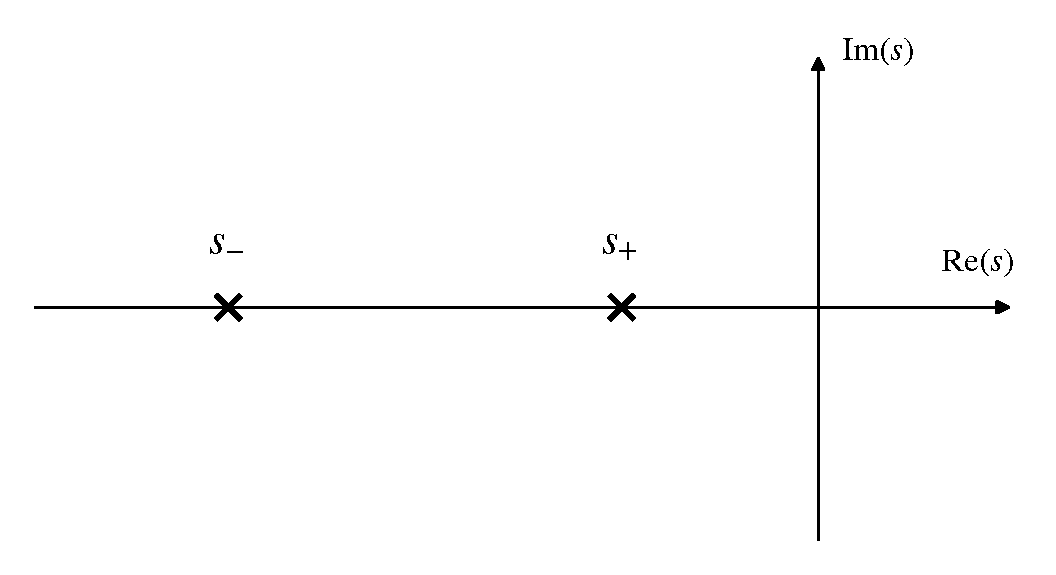
\includegraphics[height=3.3cm]{figures/overdamped_poles_symbolic.pdf}
        \caption{Two negative real poles.}
        \label{fig:overdamped-poles}
    \end{subfigure}
    \hfill
    \begin{subfigure}[t]{0.46\textwidth}
        \centering
        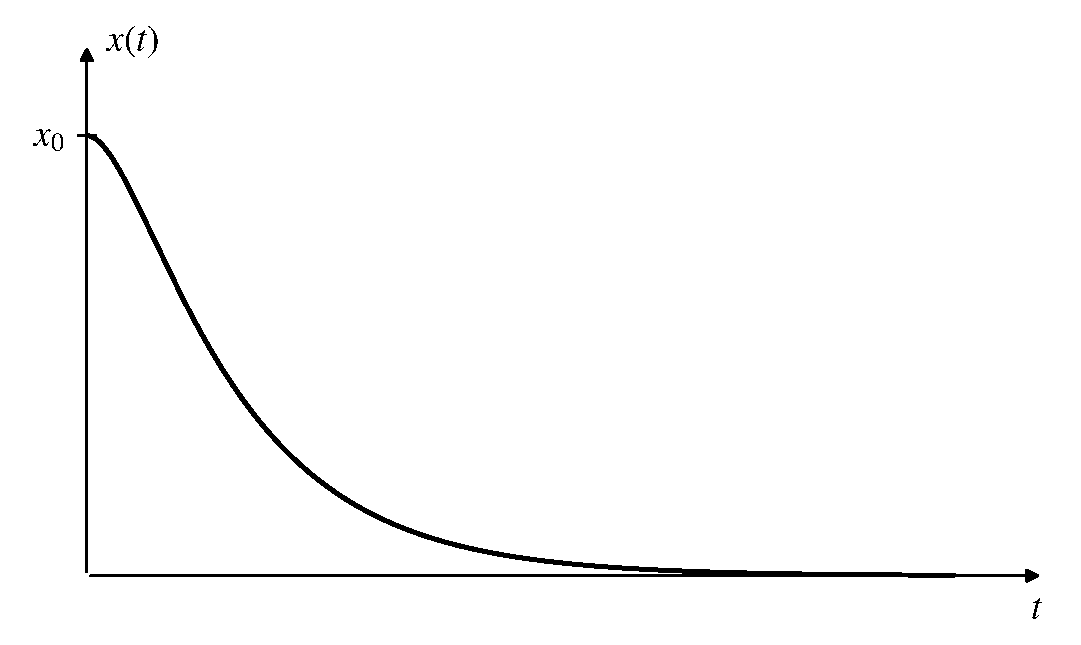
\includegraphics[height=3.3cm]{figures/overdamped_free_response.pdf}
        \caption{Non-oscillatory decay to equilibrium.}
        \label{fig:overdamped-response}
    \end{subfigure}
    \caption{Qualitative pole locations and free response in the overdamped case.}
    \label{fig:overdamped-summary}
\end{figure}

For critical damping, \(c^2=4mk\), the poles coincide. Writing
\(\alpha=c/(2m)\), the repeated pole produces a term proportional to
\(te^{-\alpha t}\), and the response is
\begin{equation}
    x_f(t)=x_0(1+\alpha t)e^{-\alpha t}.
    \label{eq:free-critical}
\end{equation}

For the underdamped case, \(c^2<4mk\), define
\[
    \omega_n=\sqrt{\frac{k}{m}},
    \qquad
    \omega_d=\sqrt{\omega_n^2-\alpha^2}.
\]
Combining the complex-conjugate terms in Equation~\eqref{eq:free-distinct}
gives the real response
\begin{equation}
    x_f(t)=x_0e^{-\alpha t}
    \left[
        \cos(\omega_dt)
        +\frac{\alpha}{\omega_d}\sin(\omega_dt)
    \right].
    \label{eq:free-underdamped}
\end{equation}
The factor \(e^{-\alpha t}\) controls the decay rate, while \(\omega_d\)
determines the oscillation frequency. This free-response analysis identifies
the transient part of the motion; evaluating vibration isolation under road
excitation additionally requires the non-zero input \(y(t)\).

\subsection{Step Response}

Consider an idealised road step \(y(t)=Y_0u(t)\), with the system at rest for
\(t<0\). Since \(Y(s)=Y_0/s\), Equation~\eqref{eq:transfer-function} gives
\begin{equation}
    X(s)=\frac{Y_0(cs+k)}{s(ms^2+cs+k)}.
    \label{eq:step-transform}
\end{equation}
The pole at \(s=0\) is introduced by the step input; the two system poles remain
\(s_+\) and \(s_-\). For distinct poles, partial fractions give
\[
    \frac{X(s)}{Y_0}
    =\frac{1}{s}
    -\frac{s_+}{s_+-s_-}\frac{1}{s-s_+}
    +\frac{s_-}{s_+-s_-}\frac{1}{s-s_-},
\]
and hence
\begin{equation}
    x(t)=Y_0\left[
        1+\frac{s_-e^{s_-t}-s_+e^{s_+t}}{s_+-s_-}
    \right].
    \label{eq:step-distinct}
\end{equation}
For critical damping this limiting expression becomes
\begin{equation}
    x(t)=Y_0\left[1+(\alpha t-1)e^{-\alpha t}\right],
    \label{eq:step-critical}
\end{equation}
whereas for the underdamped case it can be written as
\begin{equation}
    x(t)=Y_0\left\{1-e^{-\alpha t}\left[
        \cos(\omega_dt)-\frac{\alpha}{\omega_d}\sin(\omega_dt)
    \right]\right\}.
    \label{eq:step-underdamped}
\end{equation}
The final-value theorem confirms that \(x(t)\to Y_0\). The initial road jump is
an idealisation: its infinite velocity produces an impulsive damper force, so a
smooth bump would be more realistic.

\subsection{Sinusoidal Road Response}

For the causal input \(y(t)=Y_0\sin(\omega t)u(t)\),
\[
    Y(s)=\frac{Y_0\omega}{s^2+\omega^2},
    \qquad
    X(s)=\frac{Y_0\omega(cs+k)}
    {(s^2+\omega^2)(ms^2+cs+k)}.
\]
The poles \(s_\pm\) generate a decaying transient, while \(s=\pm i\omega\)
come from the forcing and generate the steady oscillation. Define
\begin{equation}
    H(i\omega)=\frac{k+ic\omega}{k-m\omega^2+ic\omega}
    =M(\omega)e^{i\phi(\omega)},
    \label{eq:frequency-response}
\end{equation}
where
\begin{align}
    M(\omega)
    &=\sqrt{\frac{k^2+c^2\omega^2}
    {(k-m\omega^2)^2+c^2\omega^2}}, \\
    \phi(\omega)
    &=\operatorname{atan2}(c\omega,k)
      -\operatorname{atan2}(c\omega,k-m\omega^2).
\end{align}
For distinct system poles, the complete zero-state response is
\begin{equation}
    x(t)=Y_0M\sin(\omega t+\phi)
    +C_+e^{s_+t}+C_-e^{s_-t},
    \label{eq:sine-complete}
\end{equation}
with
\[
    C_+=\frac{Y_0M(s_-\sin\phi-\omega\cos\phi)}{s_+-s_-},
    \qquad
    C_-=\frac{Y_0M(\omega\cos\phi-s_+\sin\phi)}{s_+-s_-}.
\]
The exponential terms vanish for \(c>0\), leaving the steady response.

Introduce the frequency ratio \(r=\omega/\omega_n\) and damping ratio
\(\zeta=c/(2m\omega_n)\). The displacement transmissibility is
\begin{equation}
    T(r)=\frac{|X|}{|Y|}
    =\sqrt{\frac{1+(2\zeta r)^2}
    {(1-r^2)^2+(2\zeta r)^2}}.
    \label{eq:transmissibility}
\end{equation}
Differentiating \(T^2\) with respect to \(r^2\) gives the peak at
\begin{equation}
    r_{\mathrm{peak}}
    =\sqrt{\frac{2}{1+\sqrt{1+8\zeta^2}}}.
    \label{eq:resonant-ratio}
\end{equation}
Thus the body follows slow road motion because \(T(0)=1\), is amplified near
resonance, and is isolated at high frequency because \(T(r)\to0\). Increasing
damping reduces the resonant peak but increases high-frequency transmission,
which exposes an engineering trade-off rather than a universally optimal value.
The phase is also physically relevant: it is close to zero at low frequency
and approaches \(-\pi/2\) at high frequency. Isolation therefore changes not
only the amplitude of the body motion but also its timing relative to the road.

\begin{figure}[htbp]
    \centering
    \begin{subfigure}[t]{0.49\textwidth}
        \centering
        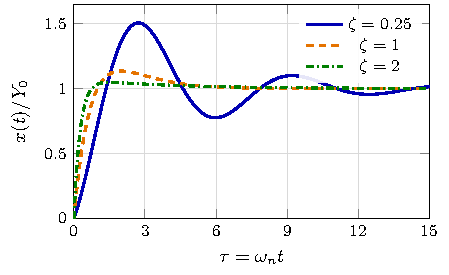
\includegraphics[height=4.2cm]{figures/step_response_comparison.pdf}
        \caption{Normalised response to a road step.}
        \label{fig:step-response-comparison}
    \end{subfigure}
    \hfill
    \begin{subfigure}[t]{0.49\textwidth}
        \centering
        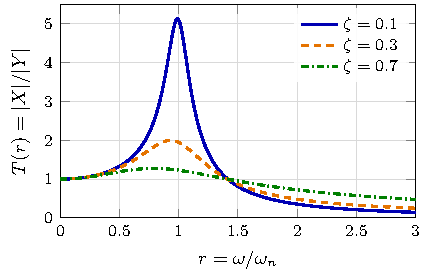
\includegraphics[height=4.2cm]{figures/sinusoidal_transmissibility.pdf}
        \caption{Sinusoidal displacement transmissibility.}
        \label{fig:sinusoidal-transmissibility}
    \end{subfigure}
    \caption{Forced-response behaviour for representative damping ratios.}
    \label{fig:forced-response-comparison}
\end{figure}

\section{Conclusion}

Starting from Newton's second law, this study derived a single-degree-of-freedom
base-excitation model and used the Laplace transform to obtain its free, step
and sinusoidal responses. For \(m,c,k>0\), the system poles lie in the left
half-plane, so all transient components decay. The step response approaches the
road height \(Y_0\), while the sinusoidal response is governed by the
displacement transmissibility \(T(r)\). Resonant amplification occurs near
\(r=1\), whereas effective vibration isolation begins when \(r>\sqrt{2}\).
Increasing damping lowers the resonant peak but increases high-frequency
transmission, demonstrating a design trade-off rather than a universally
optimal damping value. The model is limited by its linear elements, idealised
step input, and neglected tyre and wheel dynamics. A two-degree-of-freedom
quarter-car model could capture wheel-hop resonance and provide a more realistic
extension.

\end{document}
